\documentclass[11pt, a4paper]{article}

\usepackage{amsmath, amssymb, titling}
\usepackage[margin=2.75cm]{geometry}
\usepackage[colorlinks=true, linkcolor=black, urlcolor=black, citecolor=black]{hyperref}
\usepackage{graphicx}
\usepackage{float}
\usepackage{fancyhdr, lastpage}
\usepackage{xcolor}

\renewcommand\maketitlehooka{\null\mbox{}\vfill}
\renewcommand\maketitlehookd{\vfill\null}

\title{Satellite Orbit Control \\ HW3}
\author{Almog Dobrescu\\\\ID 214254252}

\pagestyle{fancy}
\cfoot{Page \thepage\ of \pageref{LastPage}}

\begin{document}

\maketitle

\thispagestyle{empty}
\newpage
\setcounter{page}{1}

\tableofcontents
\vfil
\listoffigures
\newpage

\section{Given}
\begin{equation*}
    \begin{matrix}
        T_1=100\left[min\right] = 6\cdot10^3\left[sec\right] && T_2 = T_1 = 6\cdot10^3\left[sec\right] \\
        e_1 = 0 && e_2 = 0 \\
        a_1 = \sqrt[3]{\frac{\mu T_1^2}{4\pi^2}} = 7.1366\cdot10^3\left[km\right] && a_2 = a_1 = 7.1366\cdot10^3\left[km\right]
    \end{matrix}\\
\end{equation*}
\begin{equation*}
    \alpha=\Delta i = 0.01^\circ
\end{equation*}
In CW frame with origin at Satellite \#1 and at $t=0$:
\begin{equation*}
    \begin{matrix}
    \begin{pmatrix}
        x_2(0)=0 \\ y_2(0)=-1 \\ z_2(0)=1
    \end{pmatrix}\left[\mathrm{km}\right] &&
    \begin{pmatrix}
        \dot{x}_2(0)=0 \\ \dot{y}_2(0) =0 \\ \dot{z}_2(0)=-0.74267\cdot n
    \end{pmatrix}\displaystyle\left[\frac{\mathrm{km}}{\mathrm{sec}}\right]
    \end{matrix}
\end{equation*}

\subsection{Desired}
\begin{equation*}
    \begin{matrix}
    \begin{pmatrix}
        x_2(t_f)=0 \\ y_2(t_f)=0 \\ z_2(t_f)=0
    \end{pmatrix} &&
    \begin{pmatrix}
        \dot{x}_2(t_f)=0 \\ \dot{y}_2(t_f)=0 \\ \dot{z}_2(t_f)=0
    \end{pmatrix}
    \end{matrix}
\end{equation*}

\subsection{Limitations}
The engine can't create trust in the \emph{x} direation and:
\begin{equation*}
    a_\text{max} = 8\cdot10^{-6}\left[\frac{\mathrm{km}}{\mathrm{sec}^2}\right]
\end{equation*}

\section{The CW equations}
\begin{equation}
    \left\{\begin{array}{l}
        \ddot{x}-2n\dot{y}-3n^2x=f_x\\
        \ddot{y}+2n\dot{x}=f_y\\
        \ddot{z}+n^2z=f_z
    \end{array}\right.
\end{equation}

\subsection{x-y}
\begin{equation}
    \vec{x}=\begin{pmatrix}
        x\\\dot{x}\\y\\\dot{y}
    \end{pmatrix}
\end{equation}
\begin{equation}
    \dot{\vec{x}}=F\vec{x}+G\vec{f}
\end{equation}
Where:
\begin{equation}
    \begin{matrix}
        F=\begin{pmatrix}
            0 & 1 & 0 & 0 \\
            3n^2 & 0 & 0 & 2n \\
            0 & 0 & 0 & 1 \\
            0 & -2n & 0 & 0
        \end{pmatrix} && G=\begin{pmatrix}
            0 & 0\\
            1 & 0\\
            0 & 0\\
            0 & 1
        \end{pmatrix} && f=\begin{pmatrix}
            f_x\\f_y
        \end{pmatrix}
    \end{matrix}
\end{equation}

\subsection{z}
\begin{equation}
    \vec{x}=\begin{pmatrix}
        z\\\dot{z}
    \end{pmatrix}
\end{equation}
\begin{equation}
    \dot{\vec{x}}=F\vec{x}+Gf
\end{equation}
Where:
\begin{equation}
    \begin{matrix}
        F=\begin{pmatrix}
            0 & 1 \\
            -n^2 & 0
        \end{pmatrix} && G=\begin{pmatrix}
            0 \\
            1
        \end{pmatrix} && f=\begin{pmatrix}
            f_z
        \end{pmatrix}
    \end{matrix}
\end{equation}

\subsection{x-y-z}
The equations of motion in state space form are therefor:
\begin{equation}
    \vec{x} = \begin{pmatrix}
        x\\\dot{x}\\y\\\dot{y}\\z\\\dot{z}
    \end{pmatrix}
\end{equation}
\begin{equation}
    \dot{\vec{x}}=F\vec{x}+G\vec{f}
\end{equation}
Where:
\begin{equation}
    \begin{matrix}
        F=\begin{pmatrix}
            0 & 1 & 0 & 0 & 0 & 0 \\
            3n^2 & 0 & 0 & 2n & 0 & 0 \\
            0 & 0 & 0 & 1 & 0 & 0 \\
            0 & -2n & 0 & 0 & 0 & 0 \\
            0 & 0 & 0 & 0 & 0 & 1 \\
            0 & 0 & 0 & 0 & -n^2 & 0 
        \end{pmatrix} && G=\begin{pmatrix}
            0 & 0 & 0\\
            1 & 0 & 0\\
            0 & 0 & 0\\
            0 & 1 & 0\\
            0 & 0 & 0\\
            0 & 0 & 1
        \end{pmatrix} && f=\begin{pmatrix}
            f_x\\f_y\\f_z
        \end{pmatrix}
    \end{matrix}
\end{equation}

% \begin{equation}
%     \begin{matrix}
%         \text{x-y plane:} && \text{z-direction:} \\
%         \begin{matrix}
%             x1 = x \\
%             x2 = \dot{x}
%         \end{matrix} && z1 = z \\
%         \begin{matrix}
%             y1 = y \\
%             y2 = \dot{y}
%         \end{matrix} && z2 = \dot{z}
%     \end{matrix}
% \end{equation}
% The homogeneous solution:
% \begin{equation}
%     \vec{x}(t) = \Phi_{(t,t_0)}\vec{x}_0
% \end{equation}
% \begin{equation}
%     \begin{array}{l}
%         \text{x-y plane:} \\
%         \Phi_{(t,t_0)} = \left(\begin{array}{cc|cc}
%             4-3\cos(n\tau) & 0 &\displaystyle \frac{1}{n}\sin(n\tau) &\displaystyle \frac{2}{n}\left(1-\cos(n\tau)\right) \\ 
%             6\left(\sin(n\tau)-n\tau\right) & 1 &\displaystyle \frac{2}{n}\left(\cos(n\tau)-1\right) &\displaystyle \frac{1}{n}\left(4\sin(n\tau)-3n\tau\right)\\ &&& \\ \hline &&& \\
%             3n\sin(n\tau) & 0 & \cos(n\tau) & 2\sin(n\tau) \\
%             6n\left(\cos(n\tau)-1\right) & 0 & -2\sin(n\tau) & 4\cos(n\tau)-3 
%         % \Phi_{(t,t_0)} = \left(\begin{array}{cc|cc}
%         %     \cos(n\tau) & 0 &\displaystyle \frac{1}{n}\sin(n\tau) & 0 \\ 
%         %     -2n\cos(n\tau) & 1 &\displaystyle \frac{2}{n}\left(\cos(n\tau)-1\right) &0\\ &&& \\ \hline &&& \\
%         %     -n\sin(n\tau) & 0 & \cos(n\tau) & 0 \\
%         %     -2n\cos(n\tau) & 0 & \displaystyle-\frac{2}{n}\left(n\sin(n\tau)+1\right) & 0 
%         \end{array}\right) = \begin{pmatrix}
%             \Phi_{11(t,t_0)} & \Phi_{12(t,t_0)} \\
%             \Phi_{21(t,t_0)} & \Phi_{22(t,t_0)}
%         \end{pmatrix} \\ \\ 
%     \text{z-direction:} \\
%     \Phi_{(t,t_0)} = \begin{pmatrix}
%         \cos(n\tau) & \displaystyle\frac{1}{n}\sin(n\tau) \\
%         -n\sin(n\tau) & \cos(n\tau)
%     \end{pmatrix}
%     \end{array}
% \end{equation}
% Where:
% \begin{equation*}
%     \tau = t-t_0
% \end{equation*}
% Desired:
% \begin{equation}
%     \begin{matrix}
%         \begin{pmatrix}
%             x1\\
%             y1\\
%             x2\\
%             y2
%         \end{pmatrix}(t_f) & = & \vec{0} \\\\
%         \begin{pmatrix}
%             z1\\
%             z2
%         \end{pmatrix}(t_f) & = & \vec{0}
%     \end{matrix}
% \end{equation}

\newpage
\section{case A}
The desired maneuver time is $2000\left[\mathrm{sec}\right]$. The desired approach trajectory is a straight line with constant velocity from the initial point to the origin. \\
From geometric considerations, the required velocity on the straight line is:

\begin{equation}
    \colorbox{yellow}{$\dot{\vec{x}}_{req}$} = \begin{pmatrix}
        \displaystyle\frac{x_f-x_0}{t_f}\\\\
        \displaystyle\frac{y_f-y_0}{t_f}\\\\
        \displaystyle\frac{z_f-z_0}{t_f}
    \end{pmatrix}\colorbox{yellow}{$ = \begin{pmatrix}
       0\\5\\-5
    \end{pmatrix}\cdot10^{-4}\left[\frac{\mathrm{km}}{\mathrm{sec}^2}\right]$}
\end{equation}
Which mean that the initial pulse:
\begin{equation}
    \colorbox{yellow}{$\Delta v_1 = \dot{\vec{x}}_{req} - \dot{\vec{x}}_{0} = \begin{pmatrix}
        0\\0.5\\0.2777
    \end{pmatrix}\cdot10^{-3}\left[\frac{\mathrm{km}}{\mathrm{sec}^2}\right]$}
\end{equation}
and the final pulse:
\begin{equation}
    \colorbox{yellow}{$\Delta v_f = \dot{\vec{x}}_{f} - \dot{\vec{x}}_{req} = \begin{pmatrix}
        0\\-5\\5
    \end{pmatrix}\cdot10^{-4}\left[\frac{\mathrm{km}}{\mathrm{sec}^2}\right]$}
\end{equation}



% The target trajectory:
% \begin{equation}
%     \dot{\vec{x}}_r = \underbrace{\begin{pmatrix}
%         0 & 1 & 0 & 0 & 0 & 0\\
%         0 & 0 & 0 & 0 & 0 & 0\\
%         0 & 0 & 0 & 1 & 0 & 0\\
%         0 & 0 & 0 & 0 & 0 & 0\\
%         0 & 0 & 0 & 0 & 0 & 1\\
%         0 & 0 & 0 & 0 & 0 & 0
%     \end{pmatrix}}_{\displaystyle F_r}\vec{x}_r \end{equation}
% The initial position for the approach trajectory:
% \begin{equation}
%     \vec{x}_{r(0)} = \begin{pmatrix}
%         0\\-1\\1\\
%         \displaystyle\frac{x_f-x_0}{t_f}\\
%         \displaystyle\frac{y_f-y_0}{t_f}\\
%         \displaystyle\frac{z_f-z_0}{t_f}
%     \end{pmatrix} = \begin{pmatrix}
%         0\\-1\\1\\0\\5\cdot10^{-4}\\-5\cdot10^{-4}
%     \end{pmatrix}
% \end{equation}

\noindent Since the velocity is constant:
\begin{equation*}
    \begin{pmatrix}
        \ddot{x}\\
        \ddot{y}\\
        \ddot{z}
    \end{pmatrix} = \vec{0}
\end{equation*}
By substituting the constraints in the CW equations we get:
\begin{equation}
    \left\{\begin{array}{l}
        0-2n\dot{y}=f_x\\
        0=f_y\\
        0+n^2z=f_z
    \end{array}\right.
\end{equation}
\begin{equation}
    \colorbox{yellow}{$\vec{a} = \vec{f} = \begin{pmatrix}
        -2n\cdot0.5\cdot10^{-3}\\
        0\\
        n^2z
    \end{pmatrix}$}
\end{equation}
Check that the maximum acceleration hasn't been reached:
\begin{equation}
    \begin{array}{c}
        |\vec{a}| = \sqrt{\left(2n\cdot0.5\cdot10^{-3}\right) + \left(n^2z\right)} < \sqrt{\left(2n\cdot0.5\cdot10^{-3}\right) + \left(n^2\cdot1\right)} \\\\
        |\vec{a}| < 1.5163\cdot10^{-6} < 8\cdot10^{-6} \text{\hspace{1cm}\LARGE$\surd$}
    \end{array}
\end{equation}
By solving this system numerically, we obtain the approach trajectory.
\begin{figure}[H]
    \centering
    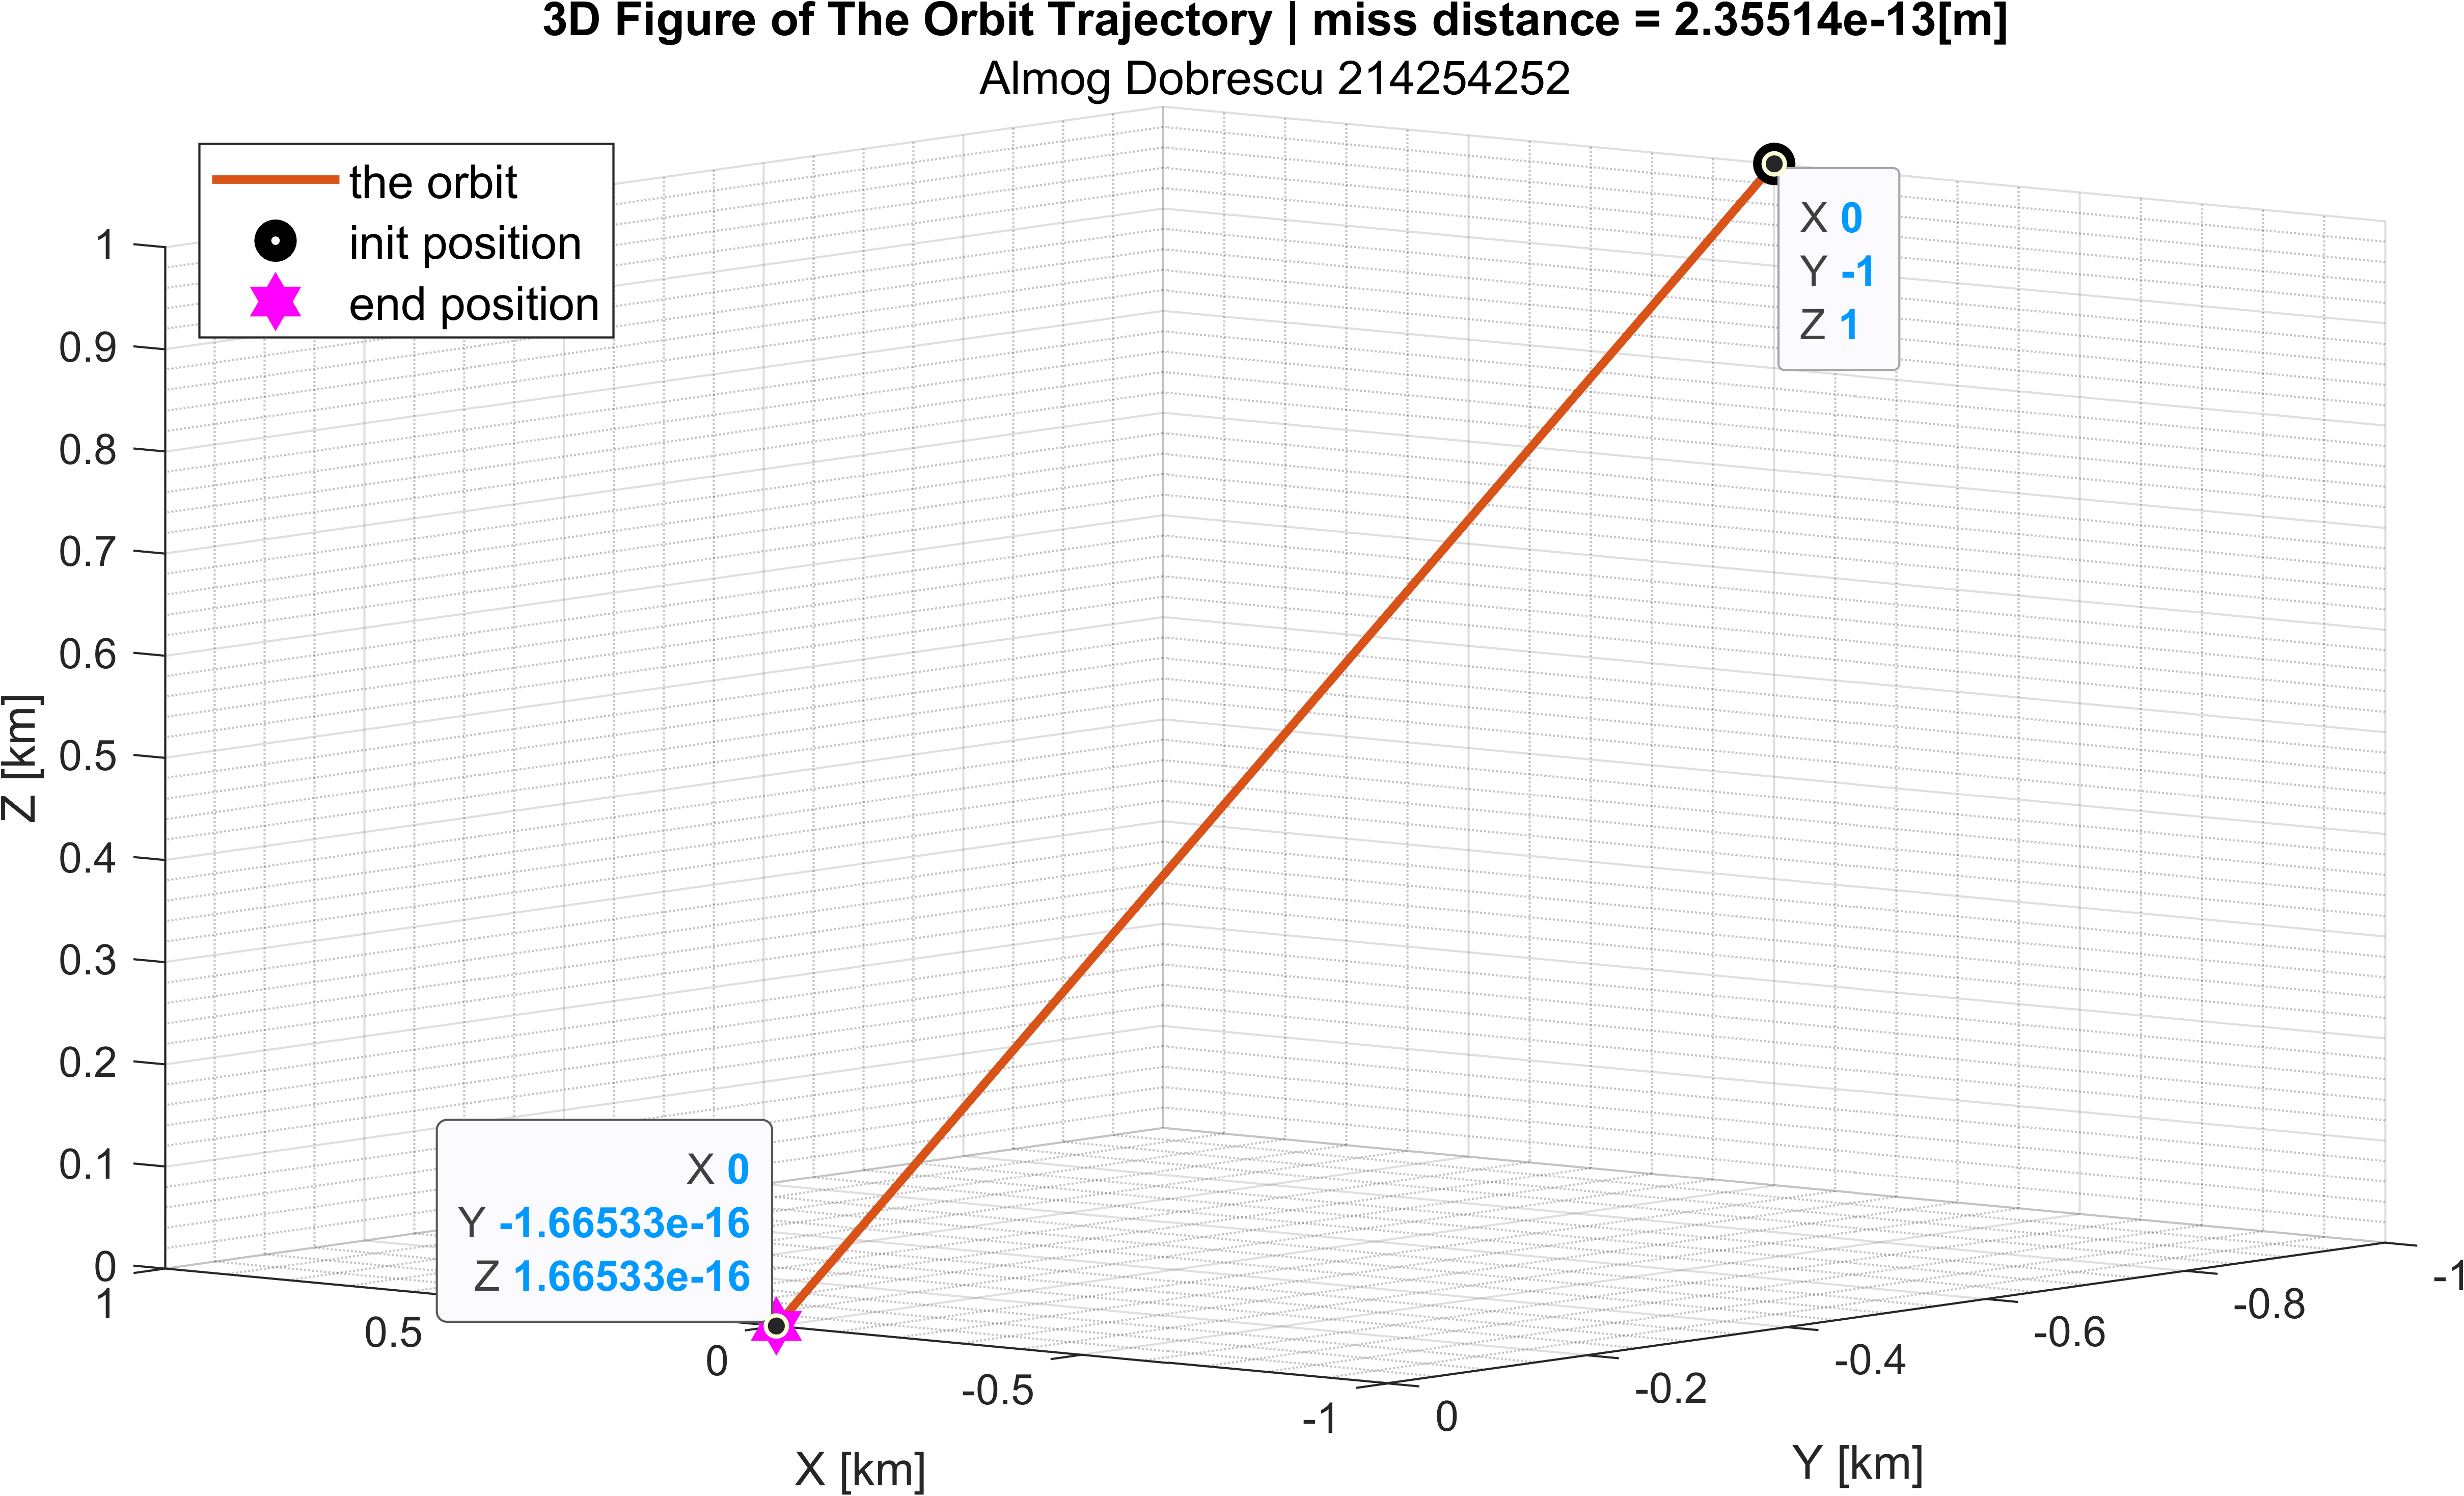
\includegraphics[width=1\textwidth]{images/graph1.png}
    \caption{3D figure of the orbit trajectory}
    \label{fig:3D-plot}
\end{figure}
\begin{figure}[H]
    \centering
    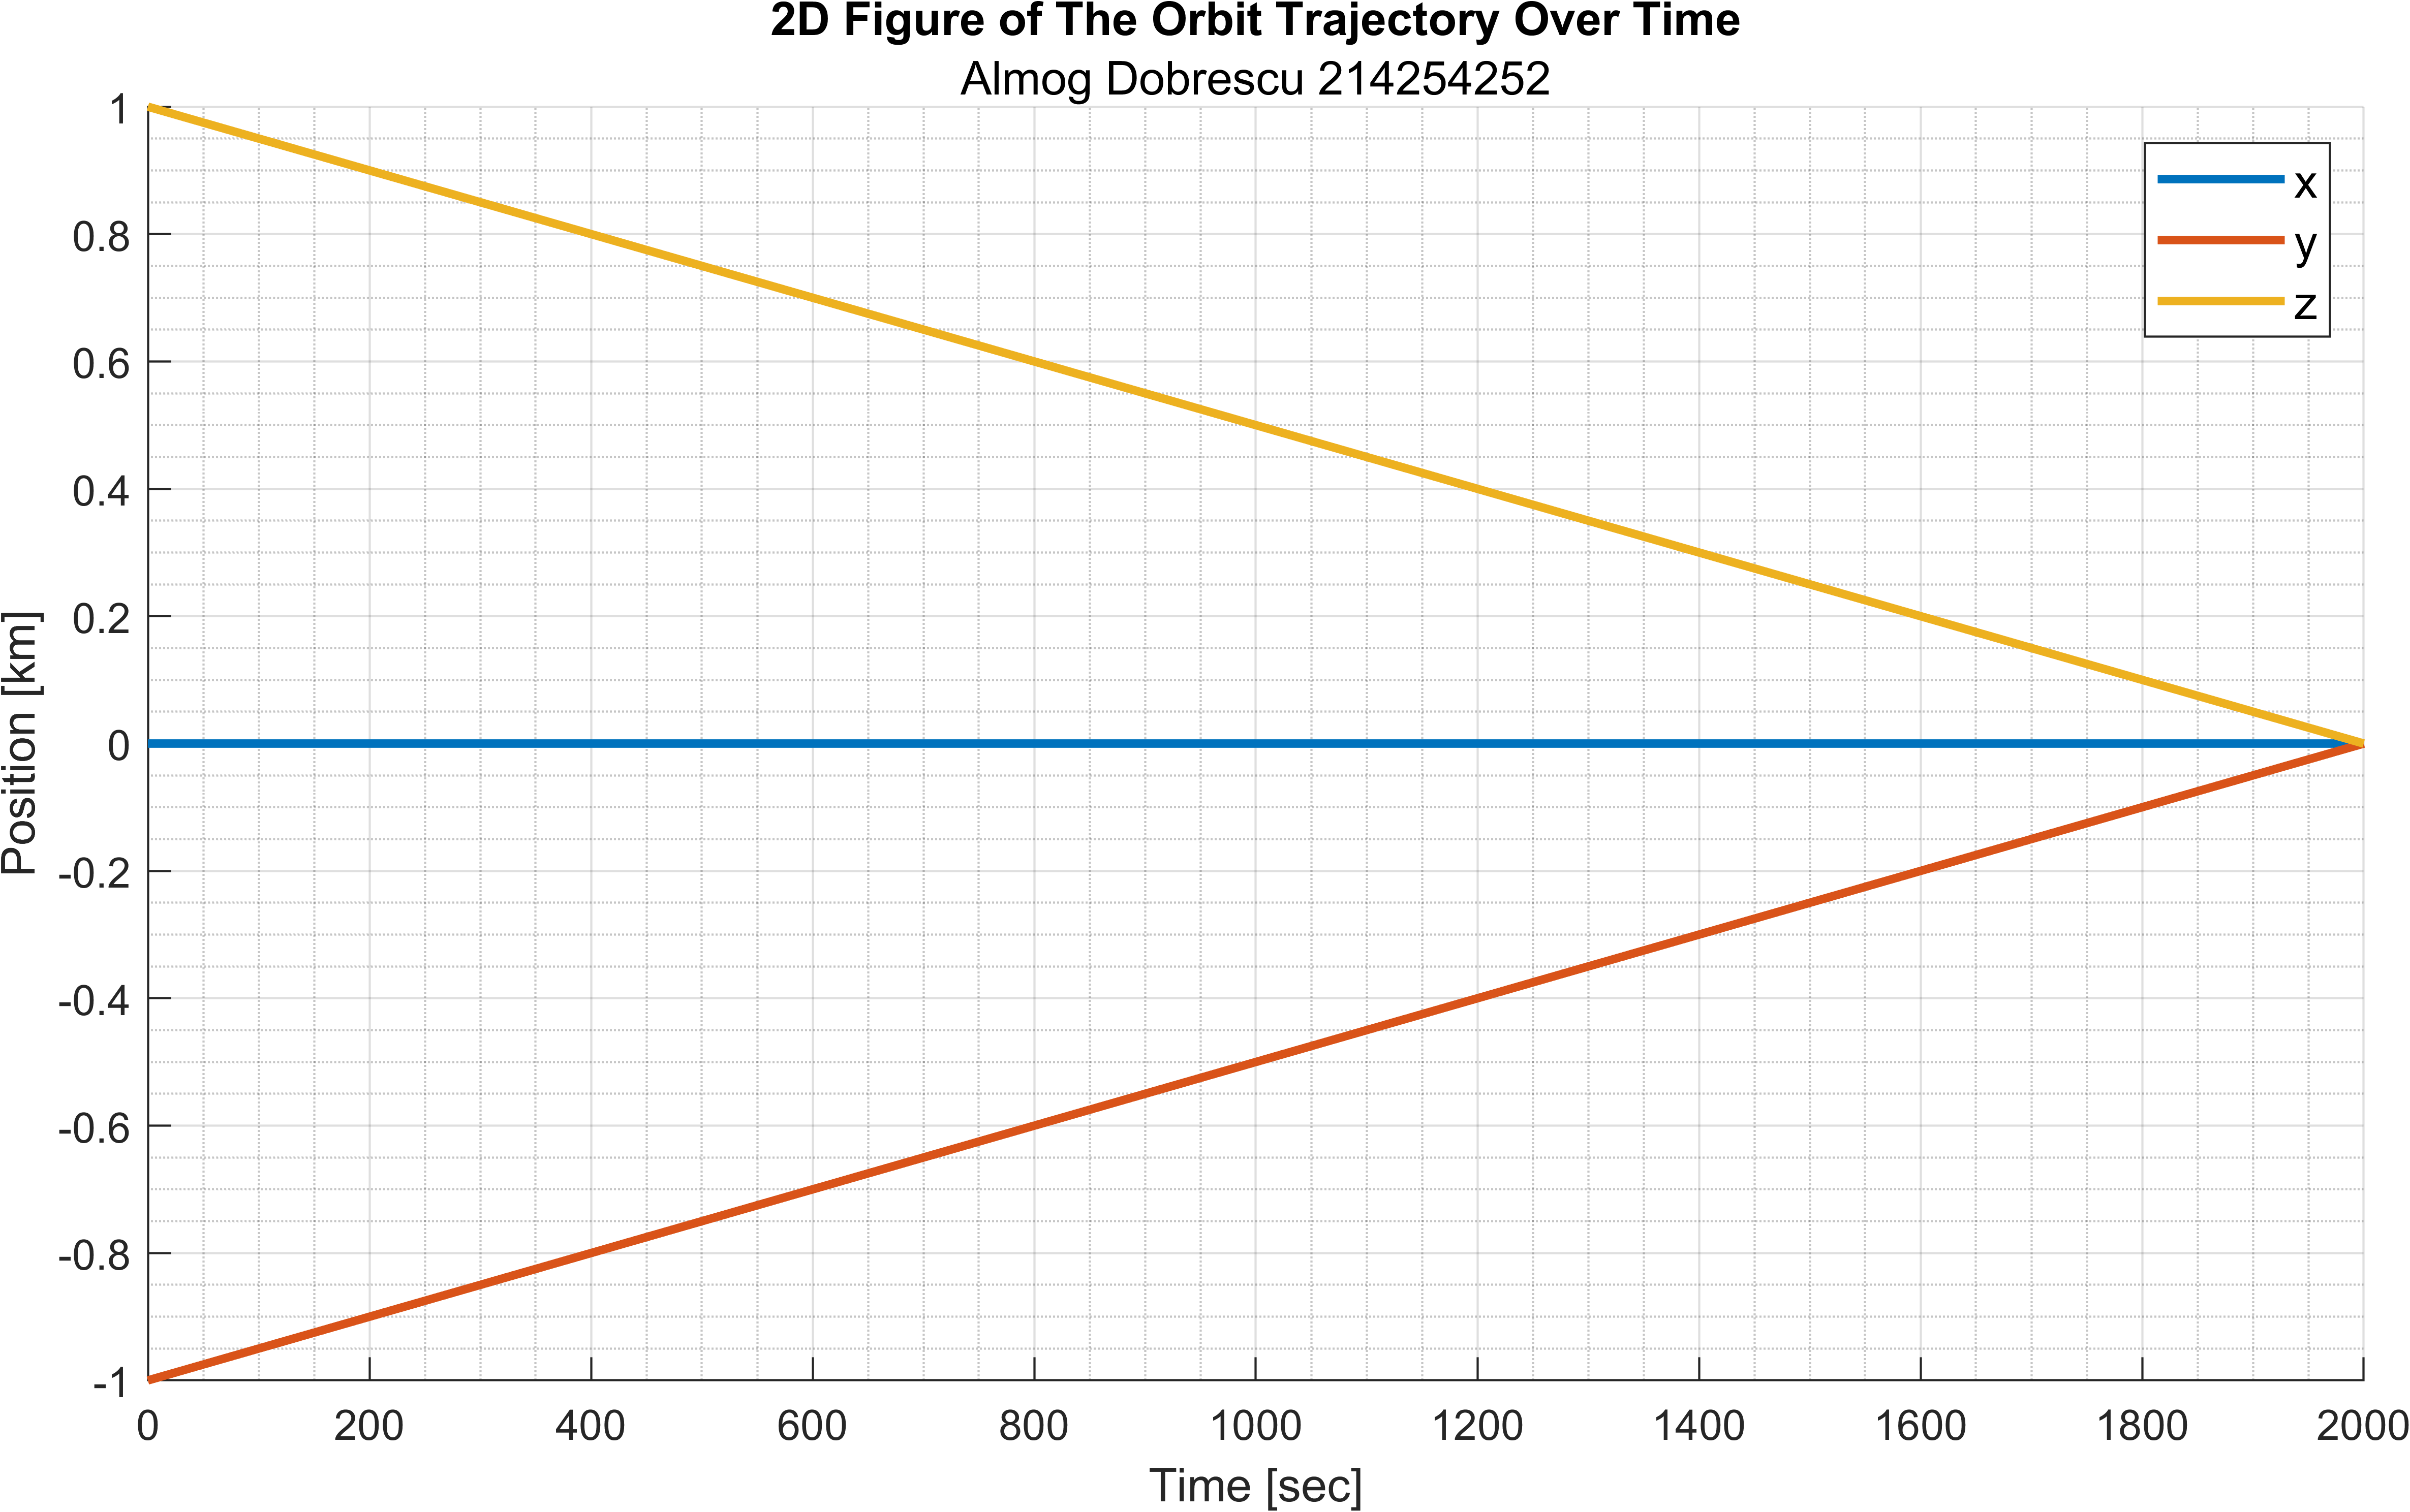
\includegraphics[width=1\textwidth]{images/graph2.png}
    \caption{2D figure of the position over time}
    \label{fig:2D-plot_over_time}
\end{figure}
\begin{figure}[H]
    \centering
    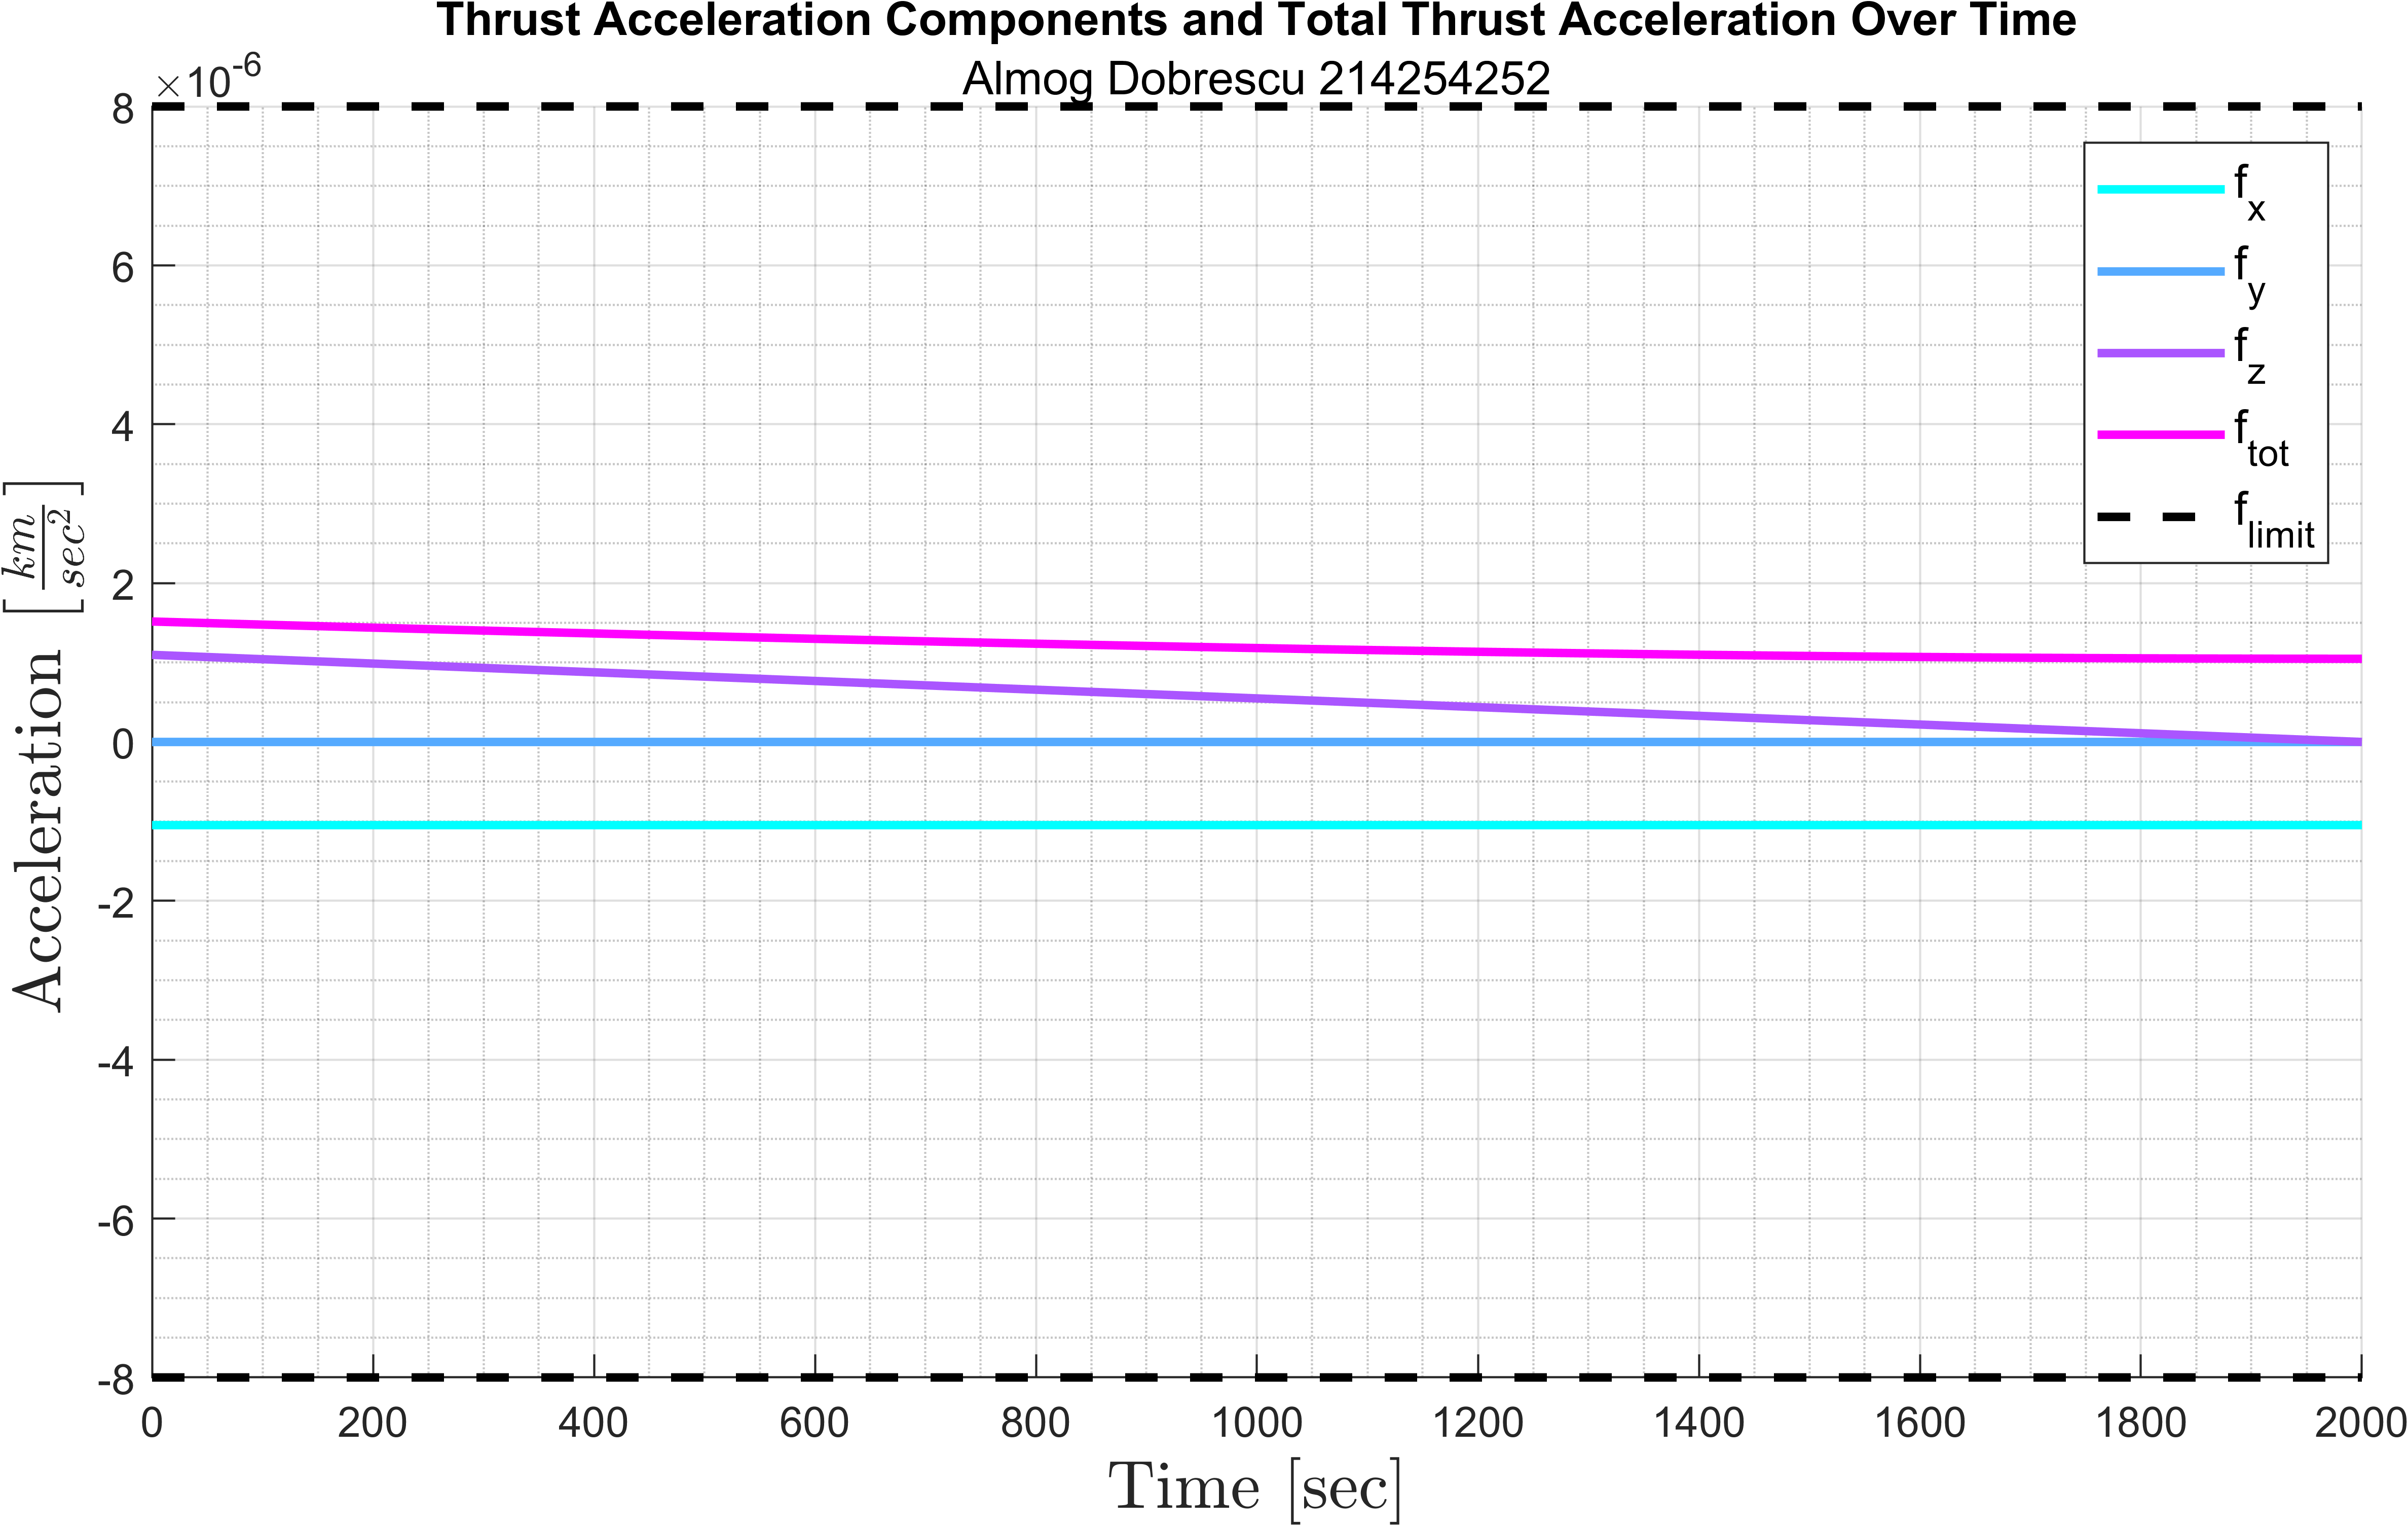
\includegraphics[width=1\textwidth]{images/graph3.png}
    \caption{Thrust acceleration components and total thrust acceleration over time}
    \label{fig:accel_over_time}
\end{figure}
\begin{figure}[H]
    \centering
    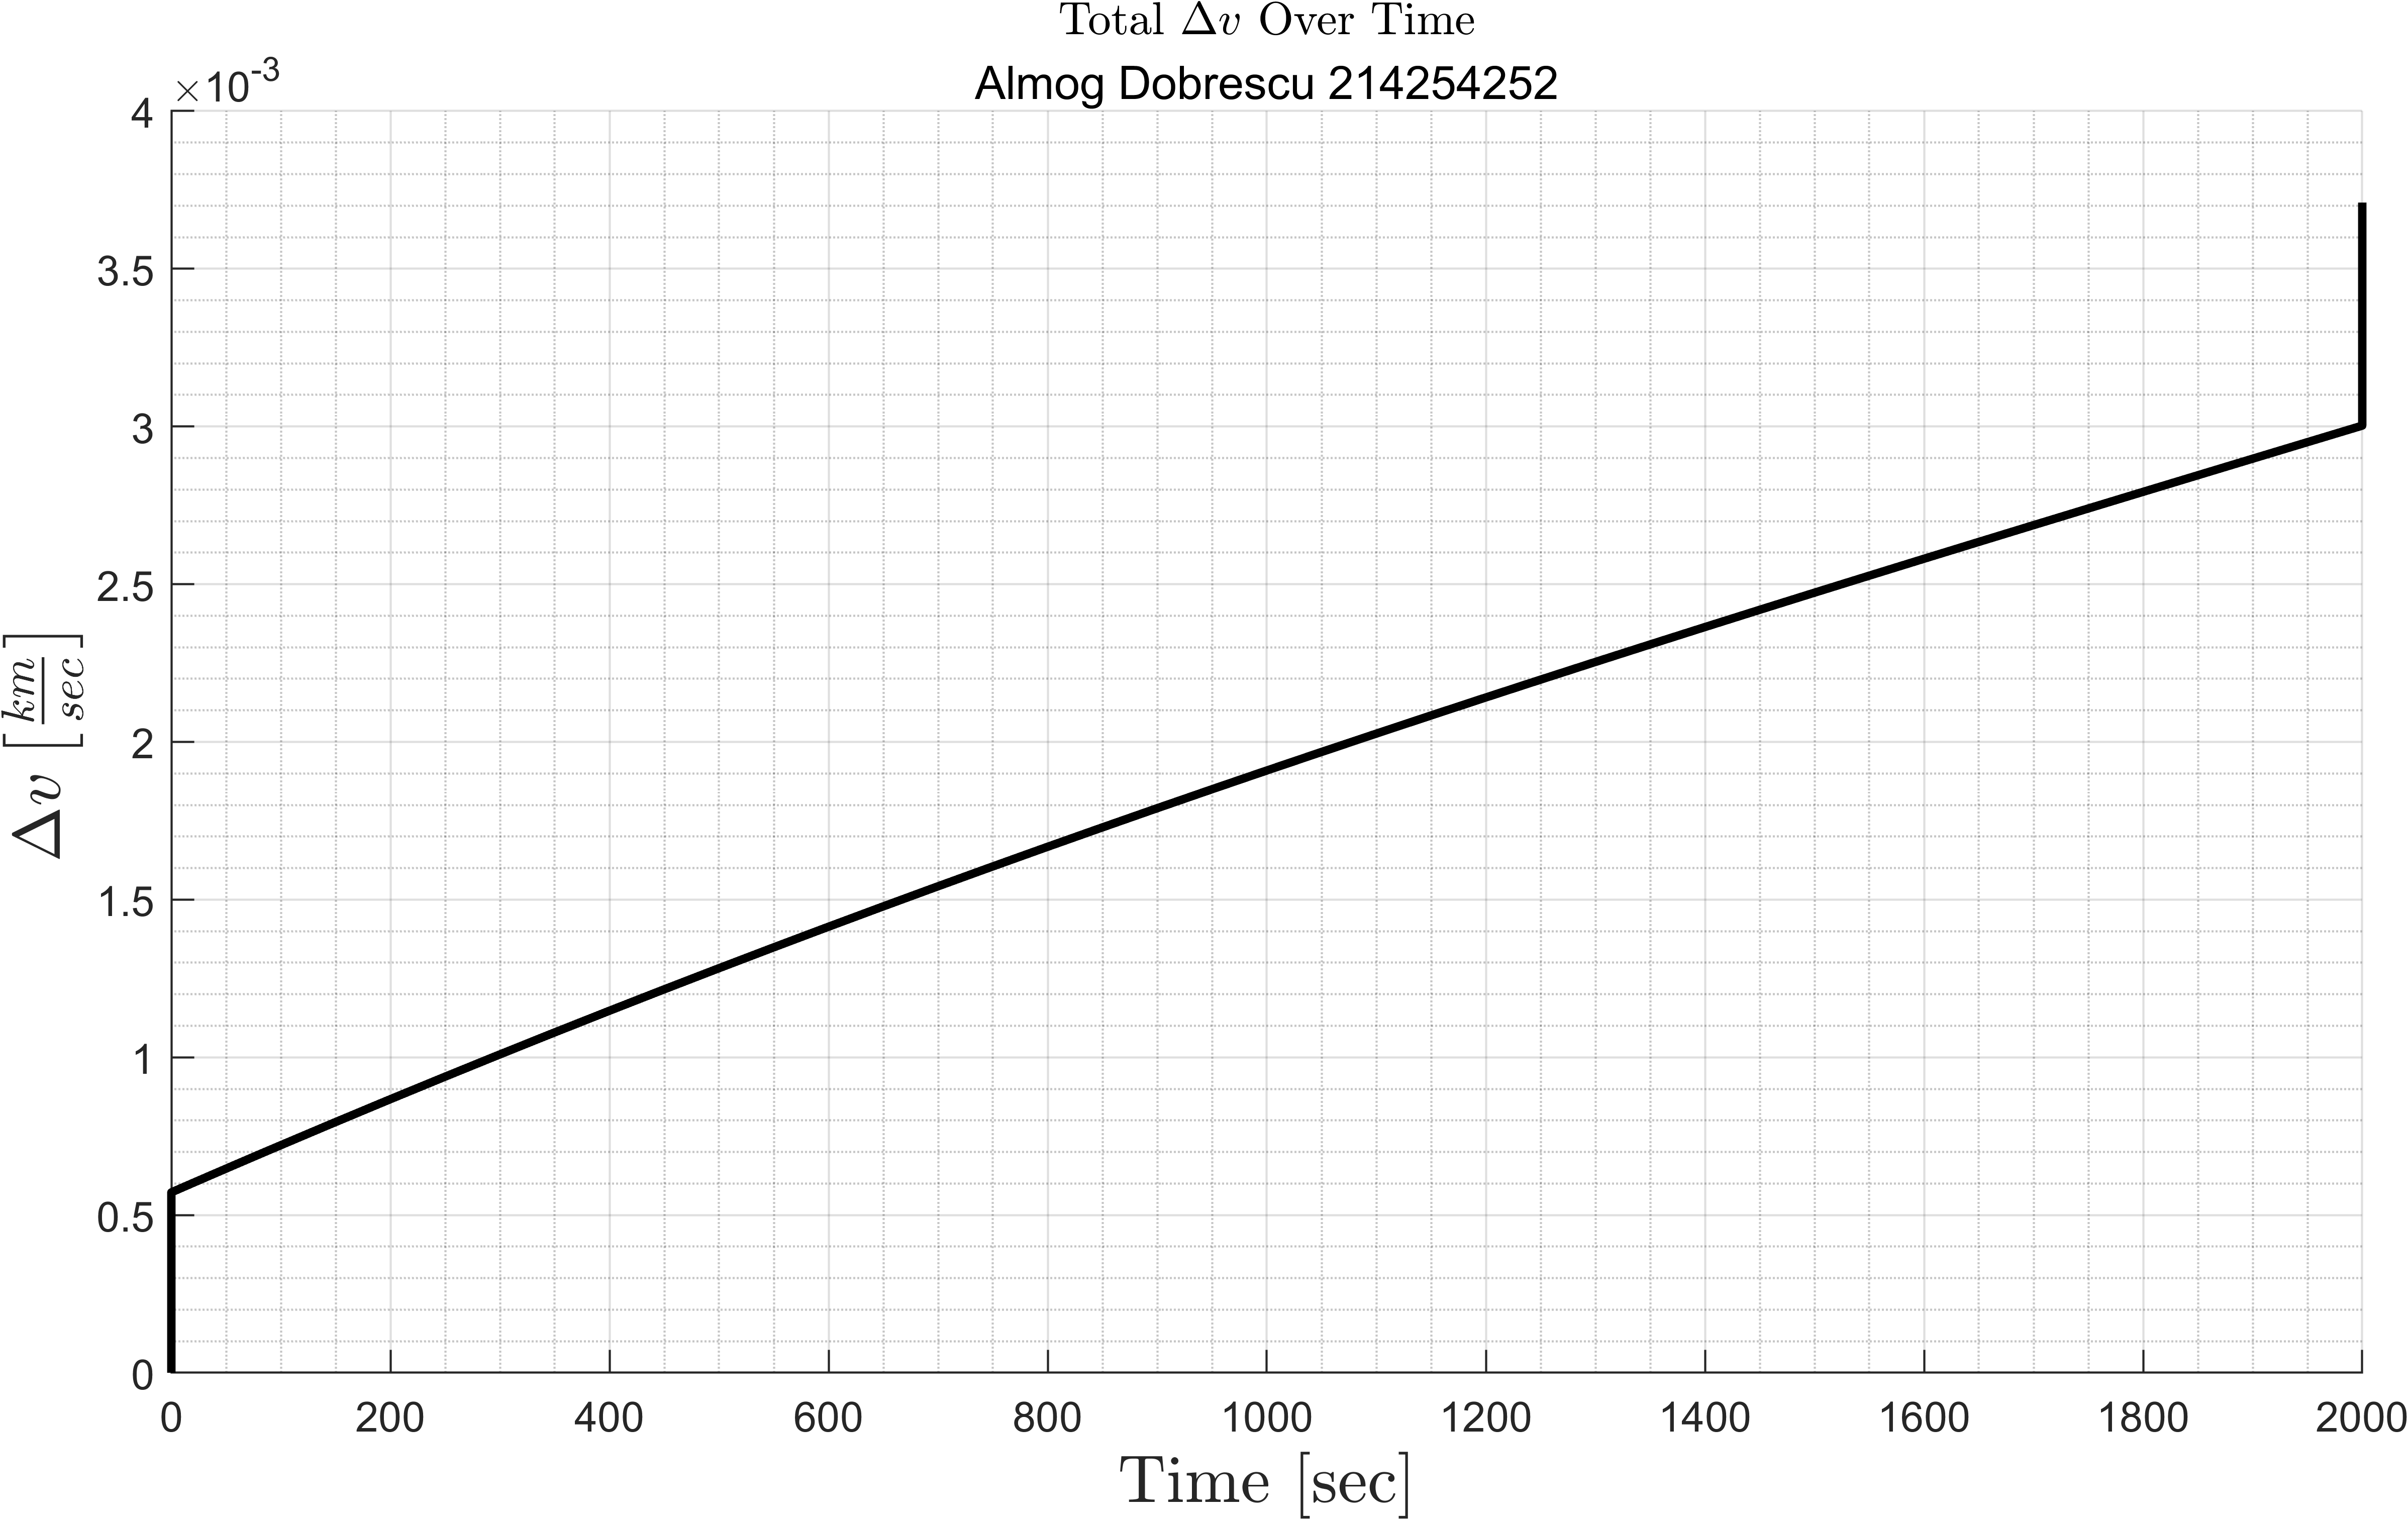
\includegraphics[width=1\textwidth]{images/graph4.png}
    \caption{Total $\Delta v$ over time}
    \label{fig:delta_v_over_time}
\end{figure}

\newpage
\section{case B}

\end{document}